\section{Methodology}

\subsection{Architecture}

\begin{figure}[h]
    \centering
      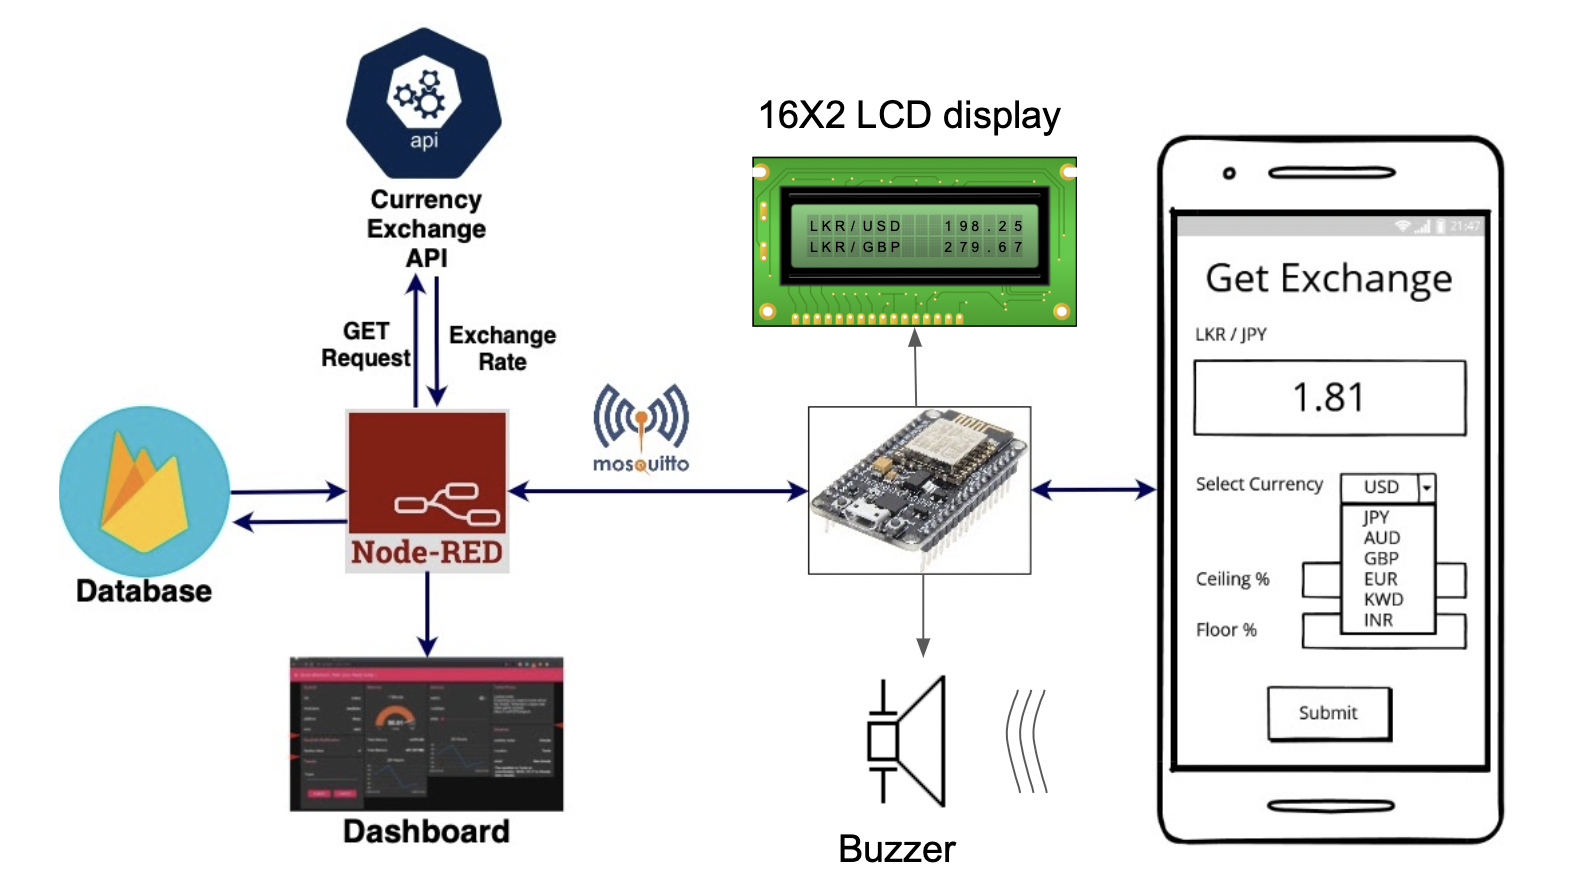
\includegraphics[width=1\textwidth]{images/arch.png}
    \caption{Architecture of the entire solution}
    \label{fig:arch}
\end{figure}

\subsection{Exchange API}

\subsection{Integrating Firebase}

\subsection{Technical analysis charts}

The hourly price data collected and stored in the real-time database can be sent through popular technical analysis functions to generate useful charts. These charts can be used to make valuable inferences. To process the price data available, an external library named TechnicalIndicators was used. Using the library, following indicators are calculated for hourly historical currency rates. Each currency will have four technical analysis charts.

\begin{enumerate}[itemsep=-1.7mm]

\item \textbf{Moving average lines} are frequently used to smooth the fluctuations in a price chart (or a chart of any time series). A moving average is simply the mean of the last n closing prices.
\item \textbf{Rate of Change oscillator} (ROC) or momentum oscillator is calculated as 100 times the difference between the latest closing price and the closing price n periods earlier. Thus, it oscillates around zero.
\item \textbf{Moving average convergence/divergence} (MACD) oscillators are drawn using exponentially smoothed moving averages, which place greater weight on more recent observations. The “MACD line” is the difference between two exponentially smoothed moving averages of the price.
\item \textbf{Relative Strength Index} (RSI) is based on the ratio of total price increases to total price decreases over a selected number of periods. This ratio is then scaled to oscillate between 0 and 100.

\end{enumerate}


\subsection{Creating the Node-Red dashboard}

\subsection{Configuring ESP8266}

\begin{figure}[h]
    \centering
      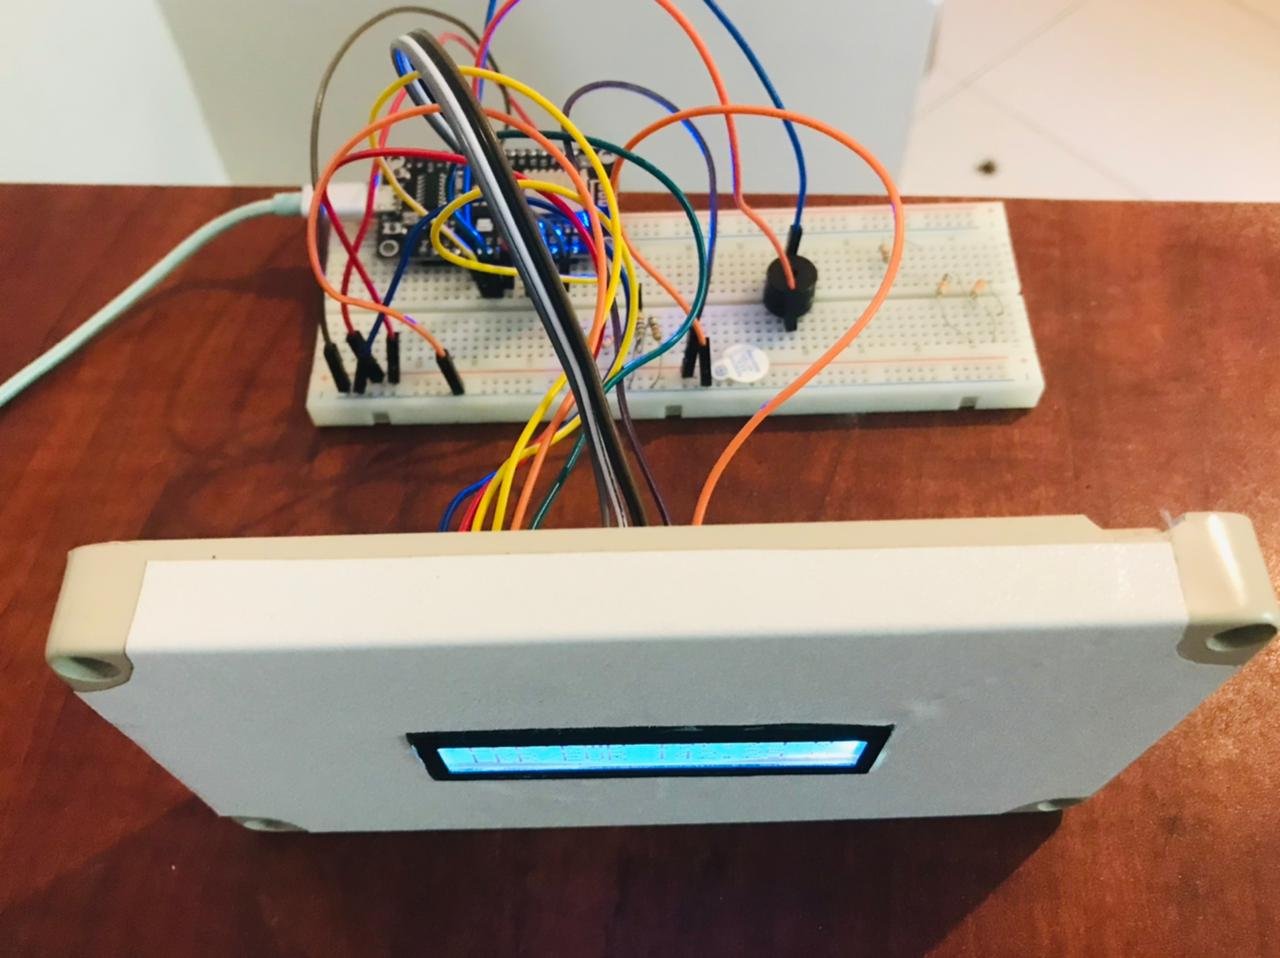
\includegraphics[width=0.7\textwidth]{images/front.png}
    \caption{Setting up ESP8266 with an LCD display and a buzzer}
    \label{front}
\end{figure}

The ESP8266 used in the IOT system performs multiple tasks to facilitate the expected functionality.

\begin{itemize}[itemsep=-1.7mm]

\item Receiving data from Node-Red through MQTT protocol
\item Decoding the compact data received to use them for the subsequent activity
\item Actively sensing alerts issued by Node-Red
\item Notifying the user with a buzzer sound when an alert is received
\item Supporting and updating the display with currency price data sent from Node-Red
\item Obtaining time and date from a NTP server to keep accurate time
\item Checking whether the received notifications are expired or not
\item Saving authentication results from the initial login in the EEPROM
\item Acting as a server to provide a login page and a web interface to select ceiling/floor limits and view current prices.
\item Sending authentication data and the data from the user interface to Node-Red through MQTT.

\end{itemize}

\subsubsection{Setting up MQTT}

When communicating through MQTT, ESP8266 subscribes to three MQTT topics.\\

\begin{lstlisting}[language=C++]
client.subscribe("IOT_6B/G05/BuzzerNotification");
client.subscribe("IOT_6B/G05/CommonData");
client.subscribe("IOT_6B/G05/AuthResponse");
\end{lstlisting}

\vspace{\baselineskip}

\textbf{IOT\_6B/G05/BuzzerNotification} sends alerts whether the ceiling price (Upper limit of acceptable prices set by the user)  or the floor price (Lower limit of acceptable prices set by the user). Given below is the format we adopted.\\


timestamp\$user\_email\$currency\$ceil\_bit\$floor\_bit\\

Eg: 1623957326\$first.lastname@gmail.com\$USD\$1\$0\\


\textbf{IOT\_6B/G05/CommonData} sends the regular currency value updates of the six currencies we have selected. Along with the message, the information whether these prices increased or decreased is also included. Given below is the format we adopted.\\

timestamp\$USD\$GBP\$JPY\$AUD\$KWD\$EUR\$100101\\

Eg: 1623921792\$200.25\$155.25\$1.82\$143.25\$197.25\$142.25\$101000

\begin{flushleft}
{\selectfont
\NumTabs{7}

\setlength{\itemindent}{0.1in}
\item timestamp 
      \tab
      :  Unix epoch time when the data is sent
\item ceil\_bit
      \tab
      :  This is set to 1 when the ceiling price is crossed, otherwise set to 0
 
\item floor\_bit
      \tab
      :  This is set to 1 when the floor price is crossed, otherwise set to 0

\item 001001
      \tab
      :  Each bit represents the six currencies. 1 represents a recent rise in price, while 0  
      
\item 
      \tab
          represents a recent reduction in price.
}

\end{flushleft}

Combining the data like this was necessary, because a set of data should be available at a certain instance. Then the LCD display can be updated with new values at once. In addition, validating the timestamp of the data for expiration is easier when the data is combined. MQTT packets are received at random times, so receiving them together makes it easier to receive the data in an organized fashion.

\subsubsection{Decoding compact received data}

The goal here is to decode this large string and update each of them in suitable variables in the ESP8266 as given below. Each data item is separated with ‘\textdollar’ marks.\\


1623921792\$200.25\$155.25\$1.82\$143.25\$197.25\$142.25\$101000\\


timestamp = 1623921792, USD = 200.25 , GBP = 155.25, JPY = 1.82, AUD = 143.25, KWD = 197.25 , EUR = 142.25\\

When a subscribed topic receives a data item, the callback function is called. The function treats the data from two topics differently by calling additional functions process\_notification and process\_data.\\

\begin{lstlisting}[language=C++]
void callback(char* topic, byte* payload, unsigned int length) {
  if (String(topic) == "IOT_6B/G05/BuzzerNotification") {
   process_notification(payload, length, 50, 5);
  }
  if (String(topic) == "IOT_6B/G05/CommonData") {
   process_data(payload, length, 70, 8);
  }
	:
	:
}
\end{lstlisting}

\vspace{\baselineskip}
Let’s take the process\_notification function for example. It splits the byte array into character arrays and then saves them in the variables treating them as separate cases. Each time the callback function is called.\\

\begin{lstlisting}[language=C++]
void process_notification(byte* payload, unsigned int length, int charlen, int numitem) {

     int digit;
     payloadstr = "";
     Serial.println();
     for (int i = 0; i < length; i++) {
       payloadstr += (char)payload[i];
     }

     char payloadstr_array[charlen];
     payloadstr.toCharArray(payloadstr_array, charlen);

     char * token = strtok(payloadstr_array, "$");
   
     for (int i = 1; i < numitem+1; i++) {
        switch (i) {
         case 1:
            timestamp = atol(token);
            Serial.print(timestamp);
            Serial.println();
            break;
	:
	:
         }
         token = strtok(NULL, "$");
     }
}
\end{lstlisting}

\subsubsection{Sensing alerts and notifying the user}

When an alert is sent through the IOT\_6B/G05/BuzzerNotification topic, the callback function instantly identifies a crossing in ceiling or floor prices to activate the buzzer. 

Checking whether the notifications are expired is essential to make sure the user is not alerted based on old information. ESP8266 was configured to have updated time and date. The timestamp attached to the notification is cross-checked against the unix epoch time available in the ESP8266. An example is given below.\\

\begin{lstlisting}[language=C++]
if (timestamp > unix_epoch - 19820) {
    current_user = String(token);
}
\end{lstlisting}

\subsubsection{Supporting the LCD 16x2 display}

LCD display is used to display the live currency prices, along with the date and time. These values are displayed one by one sequentially.


\begin{figure}[h]
    \centering
      \includegraphics[width=0.5\textwidth]{images/lcd.jpg}
    \caption{LCD display showing currency values, time and date}
    \label{lcd}
\end{figure}



The time and date was obtained using a readily available library for ESP8266 that enables the ESP8266 to communicate with an NTP (Network Time Protocol) Server.


\section{Conclusion}

